\documentclass[conference,a4paper]{IEEEtran}
\IEEEoverridecommandlockouts
\usepackage[T1]{fontenc}
\usepackage{amsmath,amssymb}
\usepackage{graphicx}
\usepackage{booktabs}
\usepackage{array}
\usepackage{multirow}
\usepackage{xcolor}
\usepackage{pifont}
\usepackage{tikz}
\usetikzlibrary{positioning,arrows.meta,fit,backgrounds,calc}
\usepackage{pgfplots}
\pgfplotsset{compat=1.17}
\usepackage[hidelinks]{hyperref}
\usepackage{cite}

\newcommand{\cmark}{\ding{51}}
\newcommand{\xmark}{\textcolor{black!35}{\ding{55}}}
\definecolor{frozen}{HTML}{E8F0FB}
\definecolor{trained}{HTML}{E3F4E6}
\definecolor{fusec}{HTML}{FDEBD8}
\definecolor{accent}{HTML}{1F5FAD}

\begin{document}

\title{Two-Stage Audio-Visual Video Anomaly Detection\\for Real-Time Surveillance\\[0.25em]{\large CS F415 Data Mining $\cdot$ Final Report $\cdot$ First Semester 2026--27}}

\author{%
\IEEEauthorblockN{Karan Bhojani}
\IEEEauthorblockA{2026H1120146P\\BITS Pilani}
\and
\IEEEauthorblockN{Nahush Kashyap M A}
\IEEEauthorblockA{2026H1120142P\\BITS Pilani}
\and
\IEEEauthorblockN{Utkarsh Shendre}
\IEEEauthorblockA{2026H1120136P\\BITS Pilani}
}

\maketitle

\begin{abstract}
Surveillance cameras record far more footage than anyone can watch, and the events worth finding are rare,
varied and labelled only at the video level. We present a cascade that runs about $10\times$ faster than real
time on a laptop and reports \emph{what} happened, \emph{when} and \emph{how confidently}. Stage~1 keeps the
weakly supervised multiple-instance-learning (MIL) ranking detector of our base paper (Sultani \emph{et al.},
CVPR 2018) but replaces its C3D features with a frozen X3D-S backbone. It scores every 2.6\,s clip and passes only
clips above a hold-out-calibrated threshold to Stage~2, where zero-shot CLIP names the event or vetoes it as
normal. A parallel audio branch, with a home-security sound head we trained on FSD50K and a zero-shot CLAP verifier,
detects off-camera screams, breaking glass, bangs, gunshots, explosions and alarms, and is fused with the video branch
per class. On a 226-video UCF-Crime test subset, Stage~1 reaches $0.843\pm0.014$ frame ROC-AUC over three seeds,
against $0.754$ reported by the base paper. The CLIP veto cuts normal videos with a false alert from 29.3\% to
22.0\% at a cost of 2.7 points of video recall. Audio adds 7.9 AP on XD-Violence, and the trained sound head raises
mAP on unseen clips from 0.41 to 0.66.
\end{abstract}

\begin{IEEEkeywords}
video anomaly detection, multiple-instance learning, weak supervision, zero-shot CLIP, audio-visual fusion
\end{IEEEkeywords}

%% ----------------------------------------------------------------------------
\section{Problem Description}
Given a camera stream (frames and audio), we want, for every anomalous event, a start and end time, a class
(\emph{burglary, fire, shooting, fighting, robbery, explosion, masked person}), a confidence and a representative
frame. Four properties make this a hard data-mining problem:
(i)~\textbf{Rarity and imbalance:} only about 5\% of frames in our test set are anomalous, so accuracy is
meaningless and false alarms dominate the operator's experience.
(ii)~\textbf{Weak labels:} frame-level annotation of hours of video is too expensive, so training receives one
label per video. This is a multiple-instance-learning setting.
(iii)~\textbf{Cost:} the detector must run live on ordinary hardware, which rules out sending every frame to a large
vision-language model.
(iv)~\textbf{Off-camera events:} some incidents, such as glass breaking in another room, are heard before they are seen.

\textbf{Contributions.} (1)~A two-stage cascade that uses the base paper's MIL detector as a cheap gate and spends
zero-shot CLIP only on the $\approx$4\% of clips it flags. (2)~A modern, light backbone (X3D-S) that gains about
nine AUC points over the base paper with an unchanged head and loss. (3)~An audio branch with a trained
home-security sound head, a CLAP verifier and per-class late fusion. (4)~A web-mining pipeline for collecting
surveillance-style video, and a local web application that explains every alert.

%% ----------------------------------------------------------------------------
\section{State of the Art}
\textbf{Base paper.} Sultani, Chen and Shah~\cite{sultani} introduced UCF-Crime (1{,}900 untrimmed videos,
128\,h, 13 anomaly types) and the formulation most later work follows. Each video is a \emph{bag} of 32 temporal
segments described by C3D features. A three-layer MLP scores each segment, and a hinge ranking loss pushes the
highest-scoring segment of an anomalous video above the highest-scoring segment of a normal one, with temporal
smoothness and sparsity terms. It reaches 75.41\% frame-level AUC and a 1.9\% frame-level false-alarm rate on
normal videos. Three gaps remain: it outputs a score but no class name, ignores audio, and relies on heavy
2015-era C3D features.

\textbf{Later work.} Table~\ref{tab:sota} summarises the field. Feature-magnitude learning (RTFM~\cite{rtfm}) and
stronger backbones push AUC into the mid-80s, and REWARD~\cite{reward} shows weakly supervised detection can run in
real time. CLIP-based methods (OVVAD~\cite{ovvad}, STPrompt~\cite{stprompt}, Flashback~\cite{flashback}) also
\emph{name} the event, at the cost of a large vision-language model applied to every snippet. Wu \emph{et
al.}~\cite{xdv} released XD-Violence and showed that audio helps, but audio is still used almost only on that
benchmark. No method in Table~\ref{tab:sota} names events, uses audio \emph{and} runs in real time on a laptop.
That combination is what we target.

\begin{table}[t]
\centering
\caption{Related work on UCF-Crime (frame AUC as reported by each paper).}
\label{tab:sota}
\setlength{\tabcolsep}{3.2pt}
\footnotesize
\begin{tabular}{@{}llcccr@{}}
\toprule
Method & Features & Names & Audio & Real & AUC \\
 & & event & & time & (\%) \\
\midrule
Sultani'18 \cite{sultani} (base) & C3D & \xmark & \xmark & \xmark & 75.41 \\
Wu'20 HL-Net \cite{xdv} & I3D (+VGGish) & \xmark & \cmark$^\dagger$ & \xmark & 82.44 \\
RTFM'21 \cite{rtfm} & I3D & \xmark & \xmark & \xmark & 84.30 \\
OVVAD'24 \cite{ovvad} & CLIP & \cmark & \xmark & \xmark & 86.40 \\
REWARD'24 \cite{reward} & UniFormer & \xmark & \xmark & \cmark & 86.94 \\
Flashback'25 \cite{flashback} & CLIP + LLM & \cmark & \xmark & \cmark & 87.30 \\
STPrompt'24 \cite{stprompt} & CLIP & \cmark & \xmark & \xmark & 88.08 \\
\midrule
\textbf{Ours} & X3D-S + CLIP & \cmark & \cmark & \cmark & 84.3$^\ast$ \\
\bottomrule
\end{tabular}\\[2pt]
\parbox{\columnwidth}{\scriptsize $^\dagger$Audio used on XD-Violence only. $^\ast$Mean of 3 seeds on our 226-video
subset (\S\ref{sec:setup}), so this is not a like-for-like ranking against full-test-set numbers.}
\end{table}

%% ----------------------------------------------------------------------------
\begin{figure*}[t]
\centering
\resizebox{\textwidth}{!}{%
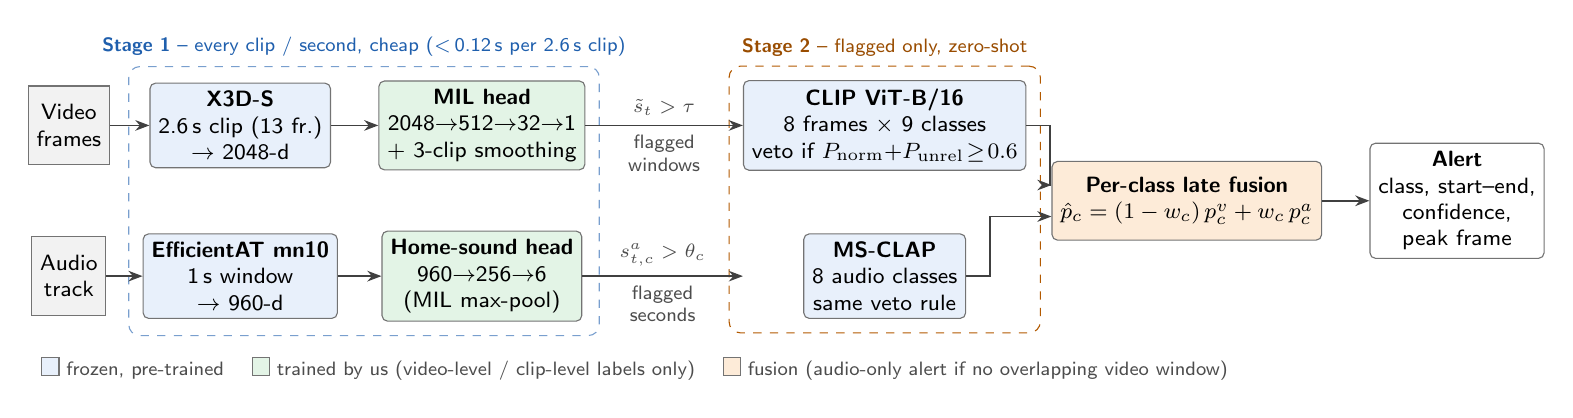
\begin{tikzpicture}[
  font=\sffamily\footnotesize,
  box/.style={draw=black!55, rounded corners=2pt, align=center, minimum height=10mm, inner sep=3pt, fill=#1},
  box/.default=white,
  io/.style={draw=black!55, align=center, minimum height=10mm, inner sep=3pt, fill=black!5},
  arr/.style={-{Stealth[length=1.8mm]}, semithick, black!75},
  lab/.style={font=\sffamily\scriptsize, text=black!70, align=center},
  node distance=4mm and 6mm]
% video row
\node[io] (vin) {Video\\frames};
\node[box=frozen, right=5mm of vin] (x3d) {\textbf{X3D-S}\\2.6\,s clip (13 fr.)\\$\to$ 2048-d};
\node[box=trained, right=6mm of x3d] (mil) {\textbf{MIL head}\\2048$\to$512$\to$32$\to$1\\+ 3-clip smoothing};
\node[box=frozen, right=20mm of mil] (clip) {\textbf{CLIP ViT-B/16}\\8 frames $\times$ 9 classes\\veto if $P_\mathrm{norm}{+}P_\mathrm{unrel}\!\ge\!0.6$};
% audio row
\node[io, below=9mm of vin] (ain) {Audio\\track};
\node[box=frozen] (eat) at (x3d |- ain) {\textbf{EfficientAT mn10}\\1\,s window\\$\to$ 960-d};
\node[box=trained] (hh) at (mil |- ain) {\textbf{Home-sound head}\\960$\to$256$\to$6\\(MIL max-pool)};
\node[box=frozen] (clap) at (clip |- ain) {\textbf{MS-CLAP}\\8 audio classes\\same veto rule};
% fusion and output
\node[box=fusec, right=7mm of $(clip.east)!0.5!(clap.east)$] (fus) {\textbf{Per-class late fusion}\\$\hat p_c=(1-w_c)\,p^{v}_c+w_c\,p^{a}_c$};
\node[box, right=6mm of fus] (out) {\textbf{Alert}\\class, start--end,\\confidence,\\peak frame};
% arrows
\draw[arr] (vin) -- (x3d);
\draw[arr] (x3d) -- (mil);
\draw[arr] (mil) -- node[lab, above]{$\tilde s_t>\tau$} node[lab, below]{flagged\\windows} (clip);
\draw[arr] (ain) -- (eat);
\draw[arr] (eat) -- (hh);
\draw[arr] (hh) -- node[lab, above]{$s^a_{t,c}>\theta_c$} node[lab, below]{flagged\\seconds} (clip.west |- hh) ;
\draw[arr] (clip.east) -- ++(3mm,0) |- ([yshift=2mm]fus.west);
\draw[arr] (clap.east) -- ++(3mm,0) |- ([yshift=-2mm]fus.west);
\draw[arr] (fus) -- (out);
% stage bands
\begin{scope}[on background layer]
\node[draw=accent!60, dashed, rounded corners=4pt, inner sep=5pt, fit=(x3d)(mil)(eat)(hh),
      label={[lab, text=accent, anchor=south]north:\textbf{Stage 1} -- every clip / second, cheap ($<$\,0.12\,s per 2.6\,s clip)}] {};
\node[draw=orange!70!black, dashed, rounded corners=4pt, inner sep=5pt, fit=(clip)(clap),
      label={[lab, text=orange!60!black, anchor=south]north:\textbf{Stage 2} -- flagged only, zero-shot}] {};
\end{scope}
% legend
\node[lab, anchor=north west] at ([yshift=-4mm]ain.south west) {%
\tikz\fill[frozen, draw=black!55] (0,0) rectangle (2.2mm,2.2mm); frozen, pre-trained \quad
\tikz\fill[trained, draw=black!55] (0,0) rectangle (2.2mm,2.2mm); trained by us (video-level / clip-level labels only) \quad
\tikz\fill[fusec, draw=black!55] (0,0) rectangle (2.2mm,2.2mm); fusion (audio-only alert if no overlapping video window)};
\end{tikzpicture}}
\caption{System overview. Both branches use a cheap trained Stage~1 gate over frozen features. Only flagged
windows reach the zero-shot Stage~2 verifiers, which name the event or veto it as normal.}
\label{fig:arch}
\end{figure*}

\section{Proposed Solution}
Fig.~\ref{fig:arch} shows the system: two branches, two stages each, joined by decision-level fusion. The guiding
idea is \emph{cost-sensitive mining}. A model with about 1\,M parameters looks at everything, and the expensive
models look only at what it flags.

\subsection{Video Stage 1: MIL ranking on X3D-S features}
Every 2.6\,s clip (13 frames sampled every 6th frame, 182\,px) is embedded by a frozen X3D-S~\cite{x3d}
(Kinetics-400, $\approx$3.8\,M parameters, $\approx$3\,GFLOPs), giving $x\in\mathbb{R}^{2048}$. For training, each
video's clips are average-pooled into $T{=}32$ L2-normalised segments, forming a bag. The head $f$ is the base
paper's MLP (2048$\to$512$\to$32$\to$1, ReLU, dropout 0.6, sigmoid; 1.07\,M parameters). For a batch of $B_a$
anomalous bags $\{a_i\}$ and $B_n$ normal bags $\{n_j\}$ we minimise the all-pairs MIL ranking loss
\begin{multline}
\mathcal{L}=\frac{1}{B_aB_n}\sum_{i,j}\max\!\bigl(0,\,1-\max_k f(a_i^k)+\max_k f(n_j^k)\bigr)\\
+\lambda_1\sum_{i,k}\bigl(f(a_i^k)-f(a_i^{k+1})\bigr)^2+\lambda_2\sum_{i,k}f(a_i^k),
\end{multline}
with $\lambda_1{=}\lambda_2{=}8{\times}10^{-5}$. The max over instances is what lets video-level labels train a
clip-level scorer. The smoothness term encodes that anomalies are temporally contiguous, and the sparsity term
encodes that they are rare. At run time each clip is scored, scores are averaged over three clips
($\tilde s_t$), consecutive clips with $\tilde s_t>\tau$ are merged into windows, and each window is padded by one
clip. The threshold $\tau$ is the largest value that keeps $\ge$90\% video-level recall on the hold-out set.

\subsection{Video Stage 2: zero-shot naming and veto with CLIP}
For a flagged window $W$, eight evenly spaced frames are embedded by CLIP ViT-B/16~\cite{clip} ($v_f$) and compared
with prompt-averaged text embeddings $t_c$ for nine classes: the seven anomalies plus \emph{normal} and
\emph{unrelated} (games, films, cartoons):
\begin{equation}
P(c\mid W)=\frac{1}{8}\sum_{f=1}^{8}\operatorname{softmax}_c\!\bigl(100\cdot\cos(v_f,t_c)\bigr).
\end{equation}
If $P(\textit{normal})+P(\textit{unrelated})\ge0.6$ the window is \emph{vetoed}. Otherwise it becomes an alert
named by its most likely anomaly class. CLIP is never trained on our data.

\subsection{Audio branch and fusion}
Each 1\,s window is embedded by a frozen EfficientAT mn10~\cite{efficientat} AudioSet model (960-d). On top we
trained a head (960$\to$256$\to$6, sigmoid) for \emph{scream, glass break, loud bang, gunshot, explosion, alarm} on
FSD50K~\cite{fsd50k}. FSD50K labels are clip-level, so this is again MIL: window scores are max-pooled per clip
before the binary cross-entropy loss. Per-class thresholds $\theta_c$ are chosen on FSD50K validation and capped at
2\% false alarms on household sounds. Flagged seconds are verified zero-shot by MS-CLAP~\cite{clap} with the same
veto rule. Where a video window and an audio event overlap, class probabilities are fused as
$\hat p_c=(1-w_c)p^v_c+w_cp^a_c$, with $w_c{=}0.5$ for shooting and explosion, $0.3$ for fighting and for the benign
classes, $0.2$ for burglary and fire, and $0$ for the visually defined classes. These weights follow the finding of
\cite{xdv} that audio helps most for acoustically salient events. A confident audio event with no overlapping
video window raises an \emph{audio-only} alert, which covers off-camera events.

\subsection{Web data mining}
To grow training data beyond UCF-Crime, we mined 489 surveillance-style video links: 367 from YouTube through
8 phrase queries with exclusions (e.g.\ \texttt{"cctv" "burglary" -movie -gta -prank}) and 122 Instagram reels through
5 hashtags (via Apify). The links were deduplicated with specific-label precedence, giving 222 burglary, 206 fire
and 60 generic-security links. A resumable labeller downloads each video, samples 16 frames, assigns CLIP class
probabilities plus a synthetic-footage score, and marks clips as \emph{use}, \emph{exclude} or \emph{review}. In a
pilot on 3 clips it correctly rejected a GTA~V video as synthetic and confirmed two burglaries. The full run and
manual review were not finished, so the mined data was \emph{not} used for training.

\subsection{Application}
A FastAPI back end with an HTML/JS front end runs every model locally (PyTorch MPS). It accepts uploaded videos or a
live camera and microphone over a WebSocket. For each alert it shows the score timeline, CLIP/CLAP class
probabilities, a per-frame anomaly curve against the veto line (Fig.~\ref{fig:ui}), and an inspector with the raw
embeddings and hidden activations.

%% ----------------------------------------------------------------------------
\begin{figure}[t]
\centering
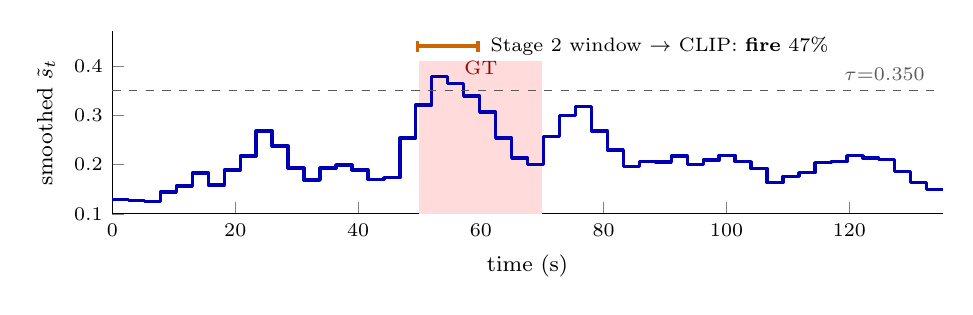
\begin{tikzpicture}
\begin{axis}[
  width=\columnwidth, height=3.9cm, xmin=0, xmax=135.2, ymin=0.10, ymax=0.47,
  xlabel={time (s)}, ylabel={smoothed $\tilde s_t$}, label style={font=\footnotesize},
  tick label style={font=\scriptsize}, ytick={0.1,0.2,0.3,0.4}, xtick={0,20,40,60,80,100,120},
  axis lines*=left, every axis plot/.append style={line join=round}, clip=false]
\fill[red!14] (axis cs:50,0.10) rectangle (axis cs:70,0.41);
\node[font=\scriptsize, text=red!60!black] at (axis cs:60,0.395) {GT};
\addplot[const plot, very thick, color=blue!70!black] coordinates {(0.0,0.1294) (2.6,0.1276) (5.2,0.125) (7.8,0.1441) (10.4,0.1565) (13.0,0.1829) (15.6,0.1581) (18.2,0.1887) (20.8,0.2173) (23.4,0.2677) (26.0,0.2372) (28.6,0.1925) (31.2,0.1682) (33.8,0.1925) (36.4,0.199) (39.0,0.189) (41.6,0.1701) (44.2,0.1732) (46.8,0.2533) (49.4,0.3204) (52.0,0.3786) (54.6,0.3646) (57.2,0.3387) (59.8,0.3063) (62.4,0.2535) (65.0,0.2129) (67.6,0.1996) (70.2,0.2567) (72.8,0.2993) (75.4,0.3181) (78.0,0.2677) (80.6,0.2294) (83.2,0.1962) (85.8,0.2062) (88.4,0.2049) (91.0,0.2171) (93.6,0.2004) (96.2,0.2089) (98.8,0.2186) (101.4,0.2057) (104.0,0.1917) (106.6,0.1635) (109.2,0.1759) (111.8,0.1834) (114.4,0.2036) (117.0,0.2057) (119.6,0.2177) (122.2,0.2132) (124.8,0.2106) (127.4,0.1862) (130.0,0.1634) (132.6,0.1488) (135.2,0.1488)};

\draw[dashed, black!65] (axis cs:0,0.3497) -- (axis cs:135.2,0.3497) node[pos=0.93, above, font=\scriptsize]{$\tau{=}0.350$};
\draw[{Bar[width=4pt]}-{Bar[width=4pt]}, very thick, orange!80!black] (axis cs:49.4,0.44) -- (axis cs:59.8,0.44)
  node[right, font=\scriptsize, text=black]{Stage 2 window $\to$ CLIP: \textbf{fire} 47\%};
\end{axis}
\end{tikzpicture}
\caption{Stage 1 scores on the unseen test video Explosion002. Only 2 of 52 clips (3.8\%) are escalated to CLIP;
the resulting window overlaps the ground-truth event (shaded).}
\label{fig:e002}
\end{figure}

\section{Experimental Setup}\label{sec:setup}
\begin{table}[t]
\centering
\caption{Datasets and how each one is used.}
\label{tab:data}
\footnotesize
\setlength{\tabcolsep}{3pt}
\begin{tabular}{@{}>{\raggedright\arraybackslash}p{1.6cm}>{\raggedright\arraybackslash}p{3.35cm}>{\raggedright\arraybackslash}p{2.85cm}@{}}
\toprule
Dataset & Size and split & Used for \\
\midrule
UCF-Crime \cite{sultani} & 1{,}000 videos (6 crime classes + normal); 697 train / 77 hold-out / 226 test (76 anom., 150 normal); 76{,}959 clips &
  Stage 1 training, choice of $\tau$ (hold-out), Stage 1 + 2 evaluation (test) \\[2pt]
XD-Violence \cite{xdv} & 4{,}754 videos, I3D + VGGish features; 3{,}954 / 800 & Value of audio fusion \\[2pt]
FSD50K \cite{fsd50k} & 11{,}143 clips (6 classes + household negatives); 6{,}374 / 998 / 3{,}771 & Audio head training, $\theta_c$ (val), evaluation \\[2pt]
RLVS, SESA & violence videos; street sounds & Fusion and CLAP sanity checks \\
\bottomrule
\end{tabular}
\end{table}

Table~\ref{tab:data} lists the data. The UCF-Crime subset keeps the six crime classes most relevant to home and
street security (arson, burglary, explosion, fighting, robbery, shooting) plus normal videos. Test videos come from
the official test split with its frame-level annotations. Stage~1 is trained with Adagrad (learning rate
$10^{-3}$, weight decay $10^{-3}$), 30 anomalous + 30 normal bags per step, for 3{,}000 steps, keeping the step
with the best hold-out video AUC, over seeds 415--417. The deployed seed 416 has $\tau{=}0.350$. The audio head
uses AdamW ($10^{-3}$, 40 epochs, 3 seeds). \textbf{No threshold or checkpoint is chosen on test data.}
\textit{Metrics:} frame-level ROC-AUC and AP; the share of normal videos with at least one alert (a video-level
false-alarm rate, stricter than the base paper's frame-level rate); CLIP top-$k$ class accuracy on true anomaly
windows; and audio mAP. Features were extracted and models trained on a Colab T4, and all inference runs on a
MacBook GPU.

%% ----------------------------------------------------------------------------
\begin{figure*}[t]
\centering
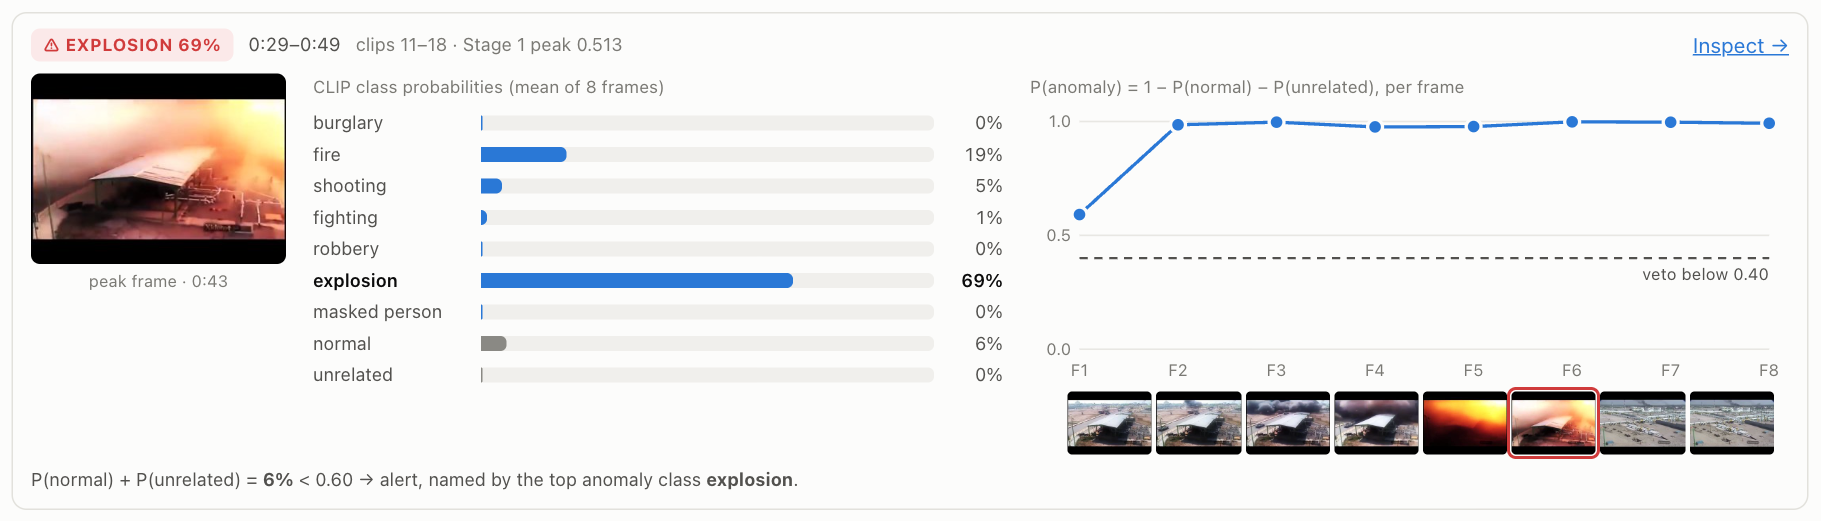
\includegraphics[width=0.92\textwidth]{ui_clipcard.png}
\caption{The application's Stage 2 view for one window of Explosion033 (video only): CLIP class probabilities
averaged over 8 frames (left) and per-frame $P(\text{anomaly})=1-P(\text{normal})-P(\text{unrelated})$ against the
veto line (right). The window is kept and named \emph{explosion} (69\%).}
\label{fig:ui}
\end{figure*}

\section{Results}

\begin{table}[t]
\centering
\caption{Stage 1 on UCF-Crime. Video-level false alarms are measured on the hold-out normals at $\tau$.}
\label{tab:stage1}
\footnotesize
\setlength{\tabcolsep}{4pt}
\begin{tabular}{@{}lcccc@{}}
\toprule
Seed & Hold-out & Test frame & Test frame & Normal videos \\
 & video AUC & AUC & AP & with alert \\
\midrule
415 & 0.887 & 0.859 & 0.206 & 42.5\% \\
416 (deployed) & 0.897 & 0.825 & 0.177 & 37.5\% \\
417 & 0.893 & 0.845 & 0.194 & 37.5\% \\
\midrule
\textbf{Mean $\pm$ std} & 0.892$\pm$.004 & \textbf{0.843$\pm$.014} & 0.192$\pm$.012 & 39.2$\pm$2.4\% \\
\bottomrule
\end{tabular}
\end{table}

\textbf{Stage 1.} Over three seeds Stage~1 reaches $0.843\pm0.014$ frame AUC (Table~\ref{tab:stage1}),
against 0.754 for the base paper. The head, loss and regularisers are the same, so we attribute most of this gain to
X3D-S replacing C3D, although the subset difference adds an unknown share. Frame AP is low (0.19) because only about
5\% of frames are anomalous. It is the metric a deployment actually feels, and the reason a second stage is needed.
At $\tau$ the gate flags 96.1\% of anomalous test videos. Fig.~\ref{fig:e002} shows why the gate is cheap: on the
unseen video Explosion002, only 2 of 52 clips cross $\tau$, and the single padded window (49.4--59.8\,s) overlaps
the ground truth (50--70\,s).


\textbf{Stage 2.} Table~\ref{tab:stage2} shows the cascade trade-off on the test set. The CLIP veto removes a
quarter of the normal videos that raised an alert (29.3\%$\to$22.0\%) and loses only two anomalous videos. On true
anomaly windows, CLIP's top-1 class is correct 34.1\% of the time (chance 14\%) and the correct class is in its top
three 70.7\% of the time (chance 43\%). Arson is the weakest class (1 of 10 correct), usually named \emph{fire} or
\emph{burglary}. These are neighbouring concepts, not random errors.

\begin{table}[t]
\centering
\caption{Effect of the zero-shot CLIP stage (UCF-Crime test, video level).}
\label{tab:stage2}
\footnotesize
\begin{tabular}{@{}lcc@{}}
\toprule
 & Stage 1 only & + CLIP veto \\
\midrule
Normal videos with an alert ($\downarrow$) & 29.3\% & \textbf{22.0\%} \\
Anomalous videos detected ($\uparrow$) & 96.1\% & 93.4\% \\
Correct class, top-1 / top-3 & -- & 34.1\% / 70.7\% \\
\bottomrule
\end{tabular}
\end{table}

\textbf{Audio.} On XD-Violence, late fusion reaches 0.681 frame AP against 0.603 for video alone and 0.606 for audio
alone (+7.9 AP), confirming that the two modalities carry complementary evidence. On RLVS, audio gives a small gain
(video AUC 0.895$\to$0.900), and CLAP alone classifies SESA sounds with 74.3\% accuracy.
Table~\ref{tab:audio} compares our trained home-sound head with zero-shot AudioSet scores on 3{,}771 unseen FSD50K
clips. It improves every class, roughly doubles AP for glass break and alarm, and lowers end-to-end false alarms on
2{,}500 household clips from 7.5\% to 5.2\%. The cost is on SESA street sounds: recall rises from 46\% to 83\%, but
false alarms on casual sounds rise from 0\% to 10\%, mostly the alarm class firing on car horns.

\begin{table}[t]
\centering
\caption{Audio Stage 1 on unseen FSD50K evaluation clips (AP). Zero-shot: AudioSet class scores; trained head: mean $\pm$ std over 3 seeds.}
\label{tab:audio}
\footnotesize
\setlength{\tabcolsep}{4pt}
\begin{tabular}{@{}lccc@{}}
\toprule
Class (positives) & Zero-shot & Trained head & $\Delta$ \\
\midrule
Scream (287) & 0.599 & 0.683$\pm$.006 & +0.08 \\
Glass break (96) & 0.420 & \textbf{0.851}$\pm$.015 & +0.43 \\
Loud bang (399) & 0.280 & 0.542$\pm$.010 & +0.26 \\
Gunshot (134) & 0.523 & 0.746$\pm$.008 & +0.22 \\
Explosion (65) & 0.324 & 0.427$\pm$.004 & +0.10 \\
Alarm (382) & 0.306 & 0.717$\pm$.009 & +0.41 \\
\midrule
\textbf{mAP} & 0.409 & \textbf{0.661$\pm$.003} & \textbf{+0.25} \\
Household false alarms (+CLAP) & 7.5\% & 5.2\% & $-$2.3 \\
\bottomrule
\end{tabular}
\end{table}

\textbf{Speed.} On a MacBook GPU, X3D-S takes 80--120\,ms per 2.6\,s clip, the MIL head under 1\,ms, CLIP about
130\,ms per \emph{flagged} window, and the audio trigger about 35\,ms per second of sound, so the pipeline runs about
$10\times$ faster than real time. Because CLIP runs on only $\approx$4\% of clips, it adds almost nothing to the
average cost. Alert latency is a few seconds, since an alert needs a complete clip plus one clip of smoothing.

\textbf{Demonstration.} (1)~\emph{Video only:} Explosion033 (unseen, audio removed) gives two \emph{explosion}
alerts (69\%, 70\%) at 0:29--0:49 and 1:00--1:45, against ground truth 0:32--0:45 and 0:52--1:45 (Fig.~\ref{fig:ui}).
(2)~\emph{Audio only:} a normal street video with an unseen scream (0:08) and breaking glass (0:18) mixed in gives two
audio-only alerts while the video score stays low. (3)~\emph{Live:} with the camera on the classroom, playing a
glass-break or siren sound from a phone raises an audio alert within about a second.


%% ----------------------------------------------------------------------------
\section{Discussion and Limitations}
\textbf{False alarms.} The base paper's 1.9\% is a \emph{frame-level} rate at a 0.5 threshold. Our 22\% is the
share of whole normal videos, often minutes long, with \emph{any} alert, at a threshold set for 90\% recall.
The two numbers are not comparable, but ours is still too high for unattended deployment. The cascade is built to
lower it, and a stricter $\tau$ or a CLIP stage fine-tuned on hold-out windows are the obvious next levers.
\textbf{Other limits.} CLIP confuses arson with burglary and explosion with fire, and eight uniformly spaced frames
under-sample long windows (Arson007 is missed). Masked-person detection is untested for lack of labelled data. Our
UCF-Crime numbers come from a 226-video subset, not the full 290-video test set. The audio head misses many door
slams and shouts and over-fires on street horns. Mined web videos still need labelling, and alerts appear only in
the app.
\textbf{Future work.} Sample CLIP frames around the Stage~1 peak, fine-tune CLIP on hold-out windows, add
street-noise negatives and a stricter alarm threshold, finish the web-mining labelling with human review, and add
push notifications.

\section{Conclusion}
Keeping the base paper's weakly supervised MIL detector as a cheap gate, with a modern backbone, gains about nine AUC
points over that paper and runs about ten times faster than real time on a laptop. Zero-shot CLIP and CLAP, applied
only to flagged windows, name events and remove a quarter of normal-video false alarms. A small trained audio head
adds detection of off-camera break-in sounds. The cascade shows that strong foundation models do not need to see
every frame to be useful.

\begin{thebibliography}{12}
\footnotesize
\setlength{\itemsep}{0pt}
\bibitem{sultani} W.~Sultani, C.~Chen, M.~Shah, ``Real-world anomaly detection in surveillance videos,'' \emph{CVPR}, 2018.
\bibitem{rtfm} Y.~Tian \emph{et al.}, ``Weakly-supervised video anomaly detection with robust temporal feature magnitude learning,'' \emph{ICCV}, 2021.
\bibitem{reward} H.~Karim, K.~Doshi, Y.~Yilmaz, ``Real-time weakly supervised video anomaly detection,'' \emph{WACV}, 2024.
\bibitem{ovvad} P.~Wu \emph{et al.}, ``Open-vocabulary video anomaly detection,'' \emph{CVPR}, 2024.
\bibitem{stprompt} P.~Wu \emph{et al.}, ``Weakly supervised video anomaly detection and localization with spatio-temporal prompts,'' \emph{ACM MM}, 2024.
\bibitem{flashback} H.~Lee \emph{et al.}, ``Flashback: Memory-driven zero-shot, real-time video anomaly detection,'' arXiv:2505.15205, 2025.
\bibitem{xdv} P.~Wu \emph{et al.}, ``Not only look, but also listen: Learning multimodal violence detection under weak supervision,'' \emph{ECCV}, 2020.
\bibitem{x3d} C.~Feichtenhofer, ``X3D: Expanding architectures for efficient video recognition,'' \emph{CVPR}, 2020.
\bibitem{clip} A.~Radford \emph{et al.}, ``Learning transferable visual models from natural language supervision,'' \emph{ICML}, 2021.
\bibitem{efficientat} F.~Schmid, K.~Koutini, G.~Widmer, ``Efficient large-scale audio tagging via transformer-to-CNN knowledge distillation,'' \emph{ICASSP}, 2023.
\bibitem{clap} B.~Elizalde, S.~Deshmukh, H.~Wang, ``Natural language supervision for general-purpose audio representations,'' \emph{ICASSP}, 2024.
\bibitem{fsd50k} E.~Fonseca \emph{et al.}, ``FSD50K: An open dataset of human-labeled sound events,'' \emph{IEEE/ACM TASLP}, 2022.
\end{thebibliography}

\end{document}
